%\documentclass[a4paper,12pt,twoside]{report}
\documentclass[a4paper,12pt]{report}


\newcommand{\bsym}[1]{\ensuremath{\boldsymbol{#1}}}
\newcommand{\bw}{\ensuremath{\bsym{w}}}
\newcommand{\bd}{\ensuremath{\bsym{d}}}
\newcommand{\bx}{\ensuremath{\bsym{x}}}
\newcommand{\bj}{\ensuremath{\bsym{j}}}
\newcommand{\bp}{\ensuremath{\bsym{p}}}
\newcommand{\bq}{\ensuremath{\bsym{q}}}
\newcommand{\bz}{\ensuremath{\bsym{z}}}
\newcommand{\bb}{\ensuremath{\bsym{b}}}
\newcommand{\by}{\ensuremath{\bsym{y}}}
\newcommand{\byy}{\ensuremath{\bsym{\tilde{y}}}}

\newcommand{\bh}{\ensuremath{\bsym{h}}}


\newcommand{\bu}{\ensuremath{\bsym{u}}}
\newcommand{\bv}{\ensuremath{\bsym{v}}}


\newcommand{\bs}{\ensuremath{\bsym{s}}}
\newcommand{\bg}{\ensuremath{\bsym{g}}}


\newcommand{\bbr}{\ensuremath{\mathcal R}}
\newcommand{\half}{\ensuremath{\frac{1}{2}}}
\newcommand{\halfhalf}{\ensuremath{\frac{1}{4}}}
\newcommand{\pointprod}[2]{\ensuremath{\left( #1 \operatorname{\prescript{}{\cdot}{\ast}} #2 \right)}}
\newcommand{\bbO}[1]{\ensuremath{\mathcal{O}\left(#1\right)}}

\usepackage{graphicx}

%\usepackage{subfig}
\usepackage{etex}
\usepackage{subcaption}
\usepackage{algpseudocode}
\usepackage{tikz,amssymb,url,amsmath,amsthm,listings,algorithm,algpseudocode,enumerate, caption, xspace, float, verbatim,tabularx,mathtools,adjustbox,pgfplots}
\pgfplotsset{width=7cm,compat=1.8}
\usepackage[pointedenum]{paralist}
\usepackage{tikz}
%\usepackage[authoryear]{natbib}
%\usepackage[sort,round,authoryear]{natbib}
\usepackage{epstopdf}
%\usepackage[breaklinks=true,pdfstartview=FitH]{hyperref}
\usepackage{times}
\usepackage{graphicx}
\usepackage{color}
\usepackage{multirow}
\usepackage{rotating}
\usepackage{bbm}
\usepackage{array}
\usepackage{latexsym}
\usepackage{longtable}
\usepackage{booktabs}
\usepackage{xr}
\usepackage{xcolor} % For color text
\usepackage{footmisc} % for author footnote
\usepackage{dsfont}
\usetikzlibrary{fit}
\usetikzlibrary{positioning}
\usetikzlibrary{math}
\usepackage{dbl12,rac0}
\usepackage{wallpaper}
\usepackage{grffile}
\usepackage{stmaryrd}

\usepackage{appendix}
\usepackage{amsfonts}
\usepackage{algorithmicx,algpseudocode}
\usepackage{makecell}
\usepackage{transparent}
\usepackage{background}

%\input{macro}

\usepackage[sorting=none,natbib=true,backend=bibtex,autocite=superscript,style=authoryear,maxcitenames=1]{biblatex}
\addbibresource{sdp.bib}
\addbibresource{thesis.bib}

% use CJKutf8 but not CJK
% see http://riemann.math.nccu.edu.tw/forum/viewtopic.php?f=5&t=666
\usepackage{CJKutf8}
%\begin{CJK*}{UTF8}{bkai}\end{CJK*}

% some infomation like title, autho etc.
% including chinese
\newcommand\cTitle{}
\newcommand\eTitle{Newton Methods for Factorization Machines }
\newcommand\myEname{Yu-Ting Huang}  % 我的姓名 (中文)
\newcommand\myCname{黃郁庭}  % 我的姓名 (中文)
\newcommand\advisorCnameA{林智仁\enskip博士} %指導教授A的姓名(中文)
\newcommand\advisorEnameA{Chih-Jen Lin, Ph.D.} %指導教授A的姓名(中文)
\newcommand\univCname{國立臺灣大學電機資訊學院} % 校名 (中文)
\newcommand\deptCname{國立臺灣大學電機資訊學院資訊工程學研究所} 
\newcommand\deptEname{Department of Graduate Institute of Computer Science and Information Engineering}
\newcommand\deptENameShort{Computer Science and Information Engineering}
\newcommand\collEname{College of Electrical Engineering and Computer Science}
\newcommand\univEname{National Taiwan University}
\newcommand\thesisEname{Master Dissertation}
\newcommand\degreeCname{碩士} %學位名 (中文)
\newcommand\degreeEname{Ms of Science} %學位名 (英文)
\newcommand\cYear{108} %口試年份 (中文、民國)
\newcommand\cMonth{00} %口試月份 (中文)
\newcommand\eYear{2019} %口試年份 (阿拉伯數字、西元)
\newcommand\eMonth{XX} %口試月份 (英文)


% http://www.math.nus.edu.sg/aslaksen/cs/cjk.html
% http://www.mandarintools.com/chardict_u8.html
\usepackage[
  bookmarks,
  bookmarksnumbered=true,
  unicode,
  breaklinks=true,
  hidelinks, %hide box
]{hyperref}
\hypersetup{%
  pdftitle={\cTitle (\eTitle)},
  pdfsubject={\cTitle (\eTitle)},
  pdfauthor={\myCname (\myEname)},
  pdfstartview=FitH,
%
% When submitting to NTU library, uncomment the following
% line to disable the border of the links.  You may also 
% want to uncomment the second line which hides bookmarks.
% These make them happy.
%
%  pdfborder={0 0 0},
%  pdfpagemode=None,
}
% must include breakurl after hyperref
% breakurl.sty is included in TeX Live 2007 standard distribution
%\usepackage{breakurl}

\captionsetup[table]{position=top}

\newtheorem{theorem}{Theorem}
\newtheorem{lemma}{Lemma}
\newtheorem{proposition}{Proposition}
%\newtheorem{corollary}{Corollary}
%\newtheorem{definition}{Definition}
%\newtheorem{assumption}{Assumption}
%{
%  \theorembodyfont{\rmfamily}
%  \newtheorem{algbreak}{Algorithm}
%}

\floatstyle{ruled}
\newfloat{Procedure}{H}{lox}
\floatname{Procedure}{Procedure}
\newfloat{Algorithm}{tb}{lox}
\floatname{Algorithm}{Algorithm}
\theoremstyle{break}

%\newcommand{\qed}{$ \Box $ \medskip}
%\newcommand{\Proof}{\noindent{\bf Proof.}~}
%\newcommand{\Index}[1]{#1\index{#1}}

%\input{macro} % pull pre-defined macros
\newboolean{thesis}
\setboolean{thesis}{true}
\newcommand{\best}{\textbf}

\newcommand{\mychapter}[1]{\chapter{#1}}
\newcommand{\mysection}[1]{\section{#1}}
\newcommand{\mysubsection}[1]{\subsection{#1}}

% watermark, from www.cmlab.csie.ntu.edu.tw/~r92045/Collection_of_LaTeX_Solutions.htm
\newcommand\WatermarkPicture{%
   \hspace{18.5cm}%
   \raisebox{-6.1576cm}{%
     \makebox[0pt][r]{
       {\transparent{0.5}\includegraphics[scale = 0.5]{watermark}}
     }
   }
}
\newcommand\insertdoi{
  \backgroundsetup{
      %contents={doi:10.6342/NTU201801837},
	  contents={},
      color=black,
      angle=0,
      position={current page.south east},
      scale=0.8,
      opacity=1,
      hshift={-3.5cm},
      vshift={1.5cm}
    }
}
% XXX should be in ntu.sty (rac0.sty?)
\def\startchineseabstractpage{%
 \newpage
 \phantomsection
 \addcontentsline{toc}{chapter}{{\large 中文摘要}}

 \hbox{ }
 \vspace{0.5in}
 \centerline{\large\CJKbold{中文摘要}}
 \vspace{0.7in}
 
 \CJKnormal % change back to normal face
}

\def\startcommiteeapproval{%
  \newpage

  \phantomsection
  \addcontentsline{toc}{chapter}{{\large 口試委員會審定書}}
  \AddToShipoutPicture*{
    \put(0,0){%
      \parbox[b][\paperheight]{\paperwidth}{%
        \vfill
        \centering
        \includegraphics[width=8.27in,height=11.69in]{signature}
        \vfill
      }
    }
  }
  \rule{0mm}{1in}
}

\DeclareMathOperator*{\diag}{diag}
\DeclareMathOperator*{\Diag}{Diag}
\DeclareMathOperator*{\vectorize}{vec}
\DeclareMathOperator*{\argmin}{arg\,min}


\begin{document}
\tikzset{%
arr/.style={draw opacity=1,
	decoration={markings,mark=at position 1
	with {\arrow[scale=2]{>}}},
	postaction={decorate}, shorten >=0.4pt,
	}
}

% Add watermark to every page
% to clear, use \ClearShipoutPicture
\AddToShipoutPicture{\AtPageUpperLeft{\WatermarkPicture}}
\insertdoi
\newcommand\cSize[1]{\noindent{\Large{#1}}\vspace{0.5cm}}
\newcommand\eSizeS[1]{\noindent{\large{#1}}\vspace{0.3cm}}
\newcommand\eSizeM[1]{\noindent{\Large{#1}}\vspace{0.4cm}}
\newcommand\eSizeL[1]{\noindent{\LARGE{#1}}}

\begin{CJK*}{UTF8}{bkai}

%\setlength\voffset{2cm}
%no page number
%next page will be page 1

\thispagestyle{empty}
\rule{0mm}{1.0cm}

% aligned to the center of the page
\begin{center}
% font size:
% \large < \Large < \LARGE < \huge < \Huge
\cSize{\deptCname}%
\par
\cSize{\degreeCname 論文}%
\par
\vspace{0.3cm}
\eSizeS{\deptEname}
\par
\eSizeS{\collEname}
\par
\eSizeM{\univEname}
\par
\eSizeM{\thesisEname}
\par
\vspace{1.5cm}
\cSize{\cTitle}
\par
\eSizeL{\eTitle\par}
\par
%\vspace{2.3cm}
\vspace{2.0cm}
\cSize{\myCname}%
\par
\eSizeL{\myEname}%
\par
%\hfill \makebox[1cm][s]{}\\
%\vspace{2.3cm}
\vspace{1.4cm}
\cSize{指導教授:\advisorCnameA}
\par
\eSizeL{Advisor: \advisorEnameA}
%\hfill \makebox[1cm][s]{}\\
\par
\vspace{1.4cm}
\noindent
\cSize{中華民國\;\cYear\;年\;\cMonth\;月}% 
\par

\eSizeL{\eMonth, \eYear}%
\end{center}
% restore the font size to normal
\normalsize

\newpage

\end{CJK*}



%%% Local Variables:
%%% coding: big5
%%% mode: latex
%%% TeX-master: thesis.tex
%%% TeX-command-default: "CJKLaTeX"
%%% End:


%\titlepage
%{\eTitle}
%{\myEname}
%{\degreeEname}
%{deptENameShort}
%{eYear}
%%\unnumberedpage

%\copyrightpage{\myEname} % Optional

%\newpage

%\thispagestyle{empty}
%\rule{0mm}{2.4mm}

\initializefrontsections
\begin{CJK*}{UTF8}{bkai}


%\startcommiteeapproval %口試委員審定書

%\dedicationpage{} % Optional

%%%\startacknowledgementspage % Optional
%%%\input{_ack}

\startchineseabstractpage
\begin{CJK*}{UTF8}{bkai}
...

\vspace{2\baselineskip}

\noindent
關鍵詞:
...

\end{CJK*}

\normalsizedbl

\startabstractpage
\input{abstract}

\vspace{2\baselineskip}
\noindent
KEYWORDS:

%block coordinate descent, one-class SVM, support vector data description
\tableofcontents % Mandatory
\end{CJK*}

\listoffigures
\listoftables
\startthechapters

% add your chapters, best way is to have separate TeX files for each
\mychapter{Introduction}\label{sec:intro}
\par Given a rating matrix $R$,  matrix factorization (MF) is a technique to find two dense matrices $U \in \bbr^{d \times M}$ and $V \in \bbr^{d \times N}$ such that $r_{m,n} \simeq \bu_m^T\bv_n$, where $\bu_m \in \bbr^d$ and $\bv_n \in \bbr^d$ are respectively the $m$th column of $U$ and the $n$th column of $V$, $d$ is the pre-specified number of latent features, and the entry $r_{m,n}$ denotes the feedback of the $m$th user on the $n$th item.  This task is achieved by solving the following non-convex problem
%To determines MF's parameters, we solve the following optimization problem.
\begin{equation}
    %\min_{U, V} \quad f(U, V)
    \min_{U,V} \quad \frac{1}{2}\sum_{(m, n) \in R}  (r_{m,n} - \bu_m^T \bv_n)^2+
    \frac{\lambda}{2} (\|U\|^2_F + \|V\|^2_F	)
    \label{eq:MF}
\end{equation}
where $(m, n) \in R$ indicates that rating $r_{m,n}$ is available, $\lambda$ is regularization coefficients for avoiding over-fitting, and $\|\cdot\|_F$ is the Frobenius norm.
%$R$ is is the rating matrix that includes the feedback of the $m$th user on $n$th item at the ($m$, $n$) entry $r_{m n}$. %The matrix factorization is technique to find two dense matrices $U \in \bbr^{d \times M}$ and $V \in \bbr^{d \times N}$ such that $r_{m,n} = \bu_m^T\bv_n$, where $\bu_m \in \bbr^d$ and $\bv_n \in \bbr^d$ are respectively the $m$th column of $U$ and the $n$th column of $V$.  
In fact, problem \eqref{eq:MF} is a special case of Factorization Machines (FM) \citep{SR10c}. The optimization problem solved by FM is as follows.
\begin{equation}
\min_{U, V} \quad f(U, V)\label{eq:reMF}
\end{equation}
where 
\begin{equation}
    f(U, V) = \frac{1}{2}\sum_{i=1}^l  \Bigl(y_i - (U \bw_i)^T (V \bh_i)\Bigr)^2+
    \frac{\lambda}{2} (\|U\|^2_F +\|V\|^2_F	)
    \label{eq:min_reMF}
\end{equation}
and $l$ is the total number of training instances. Problem \eqref{eq:min_reMF} can be considered as a regression problem, where $y_i$ is the label, and $\bh_i \in \bbr^N $ and $\bw_i \in \bbr^M$ are the feature vectors. If we let $l$ be the number of non-zero entries in $R$, the value $y_i=r_{m, n}$ be the corresponding rating from $R$,
\begin{equation}
    \bw_i=[\underbrace{0,\dots,0}_{\text{$m-1$}},1,0,\dots,0]^T
    \label{eq:wi},\text{ and}
\end{equation}
\begin{equation}
    \bh_i=[\underbrace{0,\dots,0}_{\text{$n-1$}},1,0,\dots,0]^T
    \label{eq:hi},
\end{equation}
then problem \eqref{eq:reMF} is reduced to \eqref{eq:MF}. Note that \eqref{eq:reMF} is a variant of FM proposed in \citet{MB16a}. 
One of its advantages is that the function in \eqref{eq:min_reMF} is multi-block convex. That is, if $U$ (or $V$) is fixed, then $f(U,V)$ is a convex function of $V$ (or $U$). In this work, we focus on solving the optimization  problem \eqref{eq:reMF}.

Many optimization methods have been proposed to minimize \eqref{eq:reMF}. We are particularly interested in Newton methods. \citet{WSC18a} have proposed an alternating Newton method and showed that it achieves state-of-the-art efficiency. The basic idea is to alternately switch between solving two sub-problems, each of which minimizes over one block of variables but fixes the other. Namely the first sub-problem minimizes over $U$ while keeping $V$ fixed, and the other minimizes over $V$ while keeping $U$ fixed.

Instead of alternately solving two sub-problems, naturally we ask why not minimizing $f(U,V)$ directly by the Newton method. To the best of our knowledge, no study has considered such a setting for factorization machines. In this work, we begin with developing a Newton method to solve problem \eqref{eq:reMF}. We then conduct detailed comparisons with the alternating Newton method.
\mychapter{Newton Method for Unconstrained Minimization }\label{sec:NewtonMin}
To derive the Newton method, we should re-write the function to have a vector of variables. To this end, the objective function in \eqref{eq:min_reMF} is changed to 
\begin{equation*}
f(\vectorize(U), \vectorize(V)),
\end{equation*}
where $\vectorize(\cdot)$ stacks all columns of a matrix to a vector.
For the standard Newton methods, at the $k$th iteration, we find a direction $\bs_k$ minimizing the following second-order approximation of the function value:
\begin{equation}
    \min_{\bs} \quad \frac{1}{2}\bs^T H_k \bs + \bg_k^T \bs
\label{eq:QP}
\end{equation}
where 
\begin{equation*}
H_k = \nabla^2 f(\vectorize(U_k), \vectorize(V_k))\text{ and }
\bg_k = \nabla f(\vectorize(U_k), \vectorize(V_k))
\end{equation*}
are the Hessian matrix and the gradient of $f(U_k, V_k)$, respectively.
If $H_k$ is positive definite, then \eqref{eq:QP} is equivalent to solving the following linear system:
\begin{equation}
    H_k\bs = -\bg_k
\label{eq:HLE}
\end{equation}

For non-convex objective functions, the Hessian matrix may not be positive definite. Then the solution of \eqref{eq:HLE} may not lead to a descent direction. In Section~\ref{sec:ANT} we will show that this issue occurs for our optimization problem \eqref{eq:reMF}. To obtain a descent direction, we can consider a positive-definite approximation of the Hessian matrix.

\par Now assume that $G_k$ is a positive definite approximation of the Hessian matrix. Instead of solving \eqref{eq:HLE}, we solve the following linear system to find a direction $\bs_k$.
\begin{equation}
	G_k\bs = -\bg_k
\label{eq:GLE}
\end{equation}

In practice, \eqref{eq:GLE} may not need to exactly solved. Therefore, truncated Newton methods have been introduced to approximately solve \eqref{eq:GLE}. Iterative methods such as conjugate gradient method are often used for approximately solving \eqref{eq:GLE}, so at each iteration an inner iterative process is involved. In particular, if CG is is used, at each inner iteration a matrix-vector product between $G_k$ and a vector must be conducted.

After a direction is found in our Newton method, we must decide the step size taken along that direction. A common setting is the backtracking line search. Namely, we find the largest step size $\theta\in\{1,\beta,\beta^2,\dots\}$ satisfying the following sufficient decrease condition.
Let 
\begin{equation}
\bs = \vectorize(S)
\label{eq:s}
\end{equation} 
and 
\begin{equation}
S = \begin{bmatrix} S_u & S_v \end{bmatrix}
\label{eq:susv}.
\end{equation}  
\begin{equation}
    f(U+\theta S_{u},V+\theta S_{v}) - f(U,V) \le \theta\nu {\bg}^T\vectorize(S),
    \label{eq:LineSearchRule}
\end{equation}
where $\nu\in(0,1)$ and $\beta\in(0,1)$ are pre-specified constants.
\mychapter{Newton Methods for Factorization Machines}\label{sec:NewtonFM}
To compute the gradient and Hessian of \eqref{eq:reMF}, we begin with the following properties of  the Kronecker product among matrices $A$, $B$ and $X$:
\begin{equation}
(B^T \otimes A)\vectorize(X) = \vectorize(AXB)
\label{eq:kronecker_vec}
\end{equation}
\begin{equation}
(A \otimes B)^T = A^T \otimes B^T
\label{eq:kronecker_T}.
\end{equation}
Moreover, the predicted value can be represented as
\begin{align}
(U \bw_i)^T (V \bh_i) &= (\bh_i^T \otimes (U \bw_i)^T)\vectorize(V)\label{eq:predict_UwVh_T} \\
&= (\bh_i \otimes (U \bw_i))^T\vectorize(V)
\label{eq:predict_UwVh},
\end{align}
where \eqref{eq:predict_UwVh_T} and \eqref{eq:predict_UwVh} are from \eqref{eq:kronecker_vec} and \eqref{eq:kronecker_T}, respectively.
The predicted value also can be represented as
\begin{align}
(U \bw_i)^T (V \bh_i) &= (V \bh_i)^T (U \bw_i) \nonumber \\
&= (\bw_i^T \otimes (V \bh_i)^T)\vectorize(U)\nonumber \\
&= (\bw_i \otimes (V \bh_i))^T \vectorize(U)
\label{eq:predict_VhUw}.
\end{align}
Then, we define 
\begin{equation}
\bp_i = U\bw_i ,
\bq_i = V\bh_i ,
%z_i = \bp_i^T\bq_i ,
\tilde{y}_i = \bp_i^T\bq_i,
b_i = \tilde{y}_i-y_i,
\label{eq:pqyb}
\end{equation}
the loss function 
\begin{equation*}
\xi_i = b_i^2 = \Bigl(\bp_i^T\bq_i-y_i\Bigr)^2, 
\end{equation*}
\begin{align*}
Q=[\bq_1,\dots,\bq_l] \in \bbr^{d\times l},
P=[\bp_1,\dots,\bp_l] \in \bbr^{d\times l},
\end{align*}
\begin{equation}
W=[\bw_1,\dots,\bw_l]^T \in \bbr^{l\times M},
H=[\bh_1,\dots,\bh_l]^T \in \bbr^{l\times N}.
\label{eq:WandH}
\end{equation}
\mysection{Gradient Calculation}
The gradient of \eqref{eq:reMF} is
\begin{align}
\nabla {f}(\vectorize(U, V)) = \lambda \vectorize(U,V) + \frac{1}{2}\sum_{i=1}^{l}\frac{\partial \xi_i}{\partial \tilde{y}_i}\begin{bmatrix} \frac{\partial \tilde{y}_i}{\partial \vectorize(U)} \\ \frac{\partial \tilde{y}_i}{\partial \vectorize(V)} \end{bmatrix}
\label{eq:gradUV}.
\end{align}
From \eqref{eq:predict_VhUw}, \eqref{eq:predict_UwVh} and \eqref{eq:pqyb},we define the following Jocobian of $\tilde{y}_i$ as
\begin {align}
%\bj_i = (\bw_i\otimes \bq_i, \bh_i\otimes \bp_i)
\bj_i &= \begin{bmatrix} \frac{\partial \tilde{y}_i}{\partial \vectorize(U)} \\ \frac{\partial \tilde{y}_i}{\partial \vectorize(V)} \end{bmatrix}\nonumber \\
&= \begin{bmatrix} \frac{\partial (\bw_i \otimes (V \bh_i))^T\vectorize(U)}{\partial \vectorize(U)} \\ \frac{\partial (\bh_i \otimes (U \bw_i))^T\vectorize(V)}{\partial \vectorize(V)} \end{bmatrix}\nonumber \\
&= \begin{bmatrix} \bw_i\otimes \bq_i \\ \bh_i\otimes \bp_i \end{bmatrix}
%&= \begin{bmatrix} \bw_i\otimes \bq_i \\ \bh_i\otimes \bp_i \end{bmatrix}_{(Md+Nd)\times 1}
\label{eq:Jacob}.
\end{align}
From \eqref{eq:gradUV} and \eqref{eq:Jacob}, the gradient is
\begin {align}
\nabla {f}(\vectorize(U, V)) 
&= \lambda \vectorize(U,V) + \sum_{i=1}^l b_i \bj_i\nonumber\\
&= \lambda \vectorize(U,V) + \begin{bmatrix} \sum_{i=1}^l b_i (\bw_i\otimes\bq_i) \\ \sum_{i=1}^l b_i (\bh_i\otimes\bp_i)\end{bmatrix}\label{eq:GradU_K1}\\
&= \lambda \vectorize(U,V) + \begin{bmatrix} \sum_{i=1}^l \vectorize\left(\bq_i b_i \bw_i^T \right) \\ \sum_{i=1}^l \vectorize\left(\bp_i b_i \bh_i^T \right)\end{bmatrix}\label{eq:GradU_K2}\\
&= \lambda \vectorize(U,V) + \begin{bmatrix} \vectorize\left( \sum_{i=1}^l \bq_i b_i \bw_i^T \right) \\ \vectorize\left( \sum_{i=1}^l \bp_i b_i \bh_i^T \right)\end{bmatrix}\nonumber\\
&= \lambda \vectorize(U,V) + \begin{bmatrix} \vectorize \Bigl ( Q \bigl(\diag(\bsym{b}) W \bigr)  \Bigr) \\ \vectorize \Bigl ( P \bigl(\diag(\bsym{b}) H \bigr)  \Bigr)\end{bmatrix}
\label{eq:Grad},
\end{align}
where $\diag(\bsym{b})$ is a diagonal matrix in which the $i$th diagonal element is $b_i$, and for the second term in \eqref{eq:GradU_K2} we apply \eqref{eq:kronecker_vec}. 
Usually $W$ and $H$ is highly sparse matrices. The cost of gradient calculation is
\begin{equation*}
\bbO{d\times (\text{nnz}(W)+\text{nnz}(H))},
\end{equation*}
where $\text{nnz}(\cdot)$ is the number of non-zero elements in a sparse matrix.
\par
\mysection{Hessian and Gauss-Newton Matrices}
The Hessian matrix of \eqref{eq:reMF} is 
\begin{align}
\begin{aligned}
&\frac{\partial }{\partial \vectorize(U,V)^T} \frac{\partial f}{\partial \vectorize(U,V)}\\
=&\lambda I + \sum_{i=1}^{l}\frac{\partial }{\partial \vectorize(U,V)^T} (b_i \bj_i)\\
=&\lambda I + \sum_{i=1}^{l} \Bigl( \frac{\partial }{\partial b_i^T} (b_i \bj_i) \frac{\partial b_i}{\partial \vectorize(U,V)^T} + \frac{\partial }{\partial \bj_i^T} (b_i \bj_i) \frac{\partial \bj_i}{\partial \vectorize(U,V)^T} \Bigr)\\
=&\lambda I + \sum_{i=1}^{l} \Bigl( \bj_i \frac{\partial b_i}{\partial \tilde{y}_i} \frac{\partial \tilde{y}_i}{\partial \vectorize(U,V)^T} + b_i I \frac{\partial \bj_i}{\partial \vectorize(U,V)^T} \Bigr)\\
=&\lambda I + \sum_{i=1}^{l} \bj_i \bj_i^T + \sum_{i=1}^{l} b_i \frac{\partial \bj_i}{\partial \vectorize(U,V)^T}, 
	\label{eq:H}
\end{aligned}
\end{align}
where $I$ is the identity matrix. This matrix may not be positive definite.
We remove the last term in \eqref{eq:H} and obtain the following Gauss-Newton matrix, which is positive definite.
\begin{equation}
    \begin{aligned}
    G &= \lambda I + \sum_{i=1}^{l}\bj_i\bj_i^T
    \label{eq:G}
    \end{aligned}
\end{equation}

To get the product between the Gauss-Newton matrix and a vector 
\begin{equation*}
\bs = \vectorize(S) = \begin{bmatrix}\vectorize(S_u)\\ \vectorize(S_v)\end{bmatrix}, 
\end{equation*}
from (\ref{eq:G}), (\ref{eq:Jacob}) and (\ref{eq:kronecker_vec}), we first calculate
\begin{equation}
\begin{aligned}
    z_i&= \bj_i^T \vectorize(S)\\
    &=\begin{bmatrix} \bw_i^T\otimes\bq_i^T & \bh_i^T\otimes\bp_i^T \end{bmatrix}\begin{bmatrix}\vectorize(S_u)\\ \vectorize(S_v)\end{bmatrix}\\
    &=\bq_i^T S_u \bw_i + \bp_i^T S_v \bh_i, \text{ }i=1,\dots,l
    \label{eq:DefZi},
\end{aligned}
\end{equation}
or equivalently
\begin{equation}
    \textbf{\textit{z}} = \biggl({Q^T}\odot{(WS_u^T)}+{P^T}\odot{(HS_v^T)}\biggr) \bsym{1}_{d\times 1}
    \label{eq:CalcZ},
\end{equation}
where $\odot$ is the Hadamard product (i.e., element-wise product) of two matrices.  Next, from (\ref{eq:DefZi}), (\ref{eq:G}), (\ref{eq:Jacob}), (\ref{eq:s}) and  (\ref{eq:kronecker_vec}),
\begin{align}
    G \bs         &= \lambda \vectorize(S) + \sum_{i=1}^l z_i \bj_i \nonumber\\
                  &= \lambda \vectorize(S) + \sum_{i=1}^l z_i \begin{bmatrix} \bw_i\otimes \bq_i \\ \bh_i\otimes \bp_i \end{bmatrix} \nonumber \\
                  &= \lambda \vectorize(S) +  \sum_{i=1}^l \begin{bmatrix}\vectorize\left(z_i \bq_i \bw_i^T\right) \\ \vectorize\left(z_i \bp_i \bh_i^T\right)\end{bmatrix} \nonumber  \\
                  &= \lambda \vectorize(S) +  \begin{bmatrix}\vectorize \Bigl ( Q \bigl(\diag(\textbf{\textit{z}}) W \bigr) \Bigr)\\\vectorize \Bigl ( P \bigl ( \diag(\textbf{\textit{z}}) H \bigr) \Bigr)\end{bmatrix} \label{eq:Hv}.
\end{align}

We investigate the complexity of the Hessian-vector product. The first term of 
\eqref{eq:Hv} is a standard vector scaling that costs \bbO{(M+N) \times d}.
For the second term in (\ref{eq:Hv}), we separately consider two major steps:
\begin{enumerate}
    \item The computation of $WS_u^T$ and $HS_v^T$: $\bbO{d \times (\text{nnz}(W)+\text{nnz}(H))}$
    \item The element-wise product between $P^T$ and $HS_v^T$:  $\bbO{ d \times l}$
    \item The product between dense vector $Q$ and $\diag{(\bsym{z})}W$: $\bbO{d \times l}$
\end{enumerate}
Therefore, the cost of one Hessian-vector  is $\bbO{d \times (\text{nnz}(W)+\text{nnz}(H)})$. 
\mysection{Implementation of Line Search}
\label{sec:implementLS}
Recalculating the function value at each $U+\theta S_{u}$ and $V+\theta S_{v}$ is expensive, where the main cost is on calculating $((U+\theta S_{u})\bw_i)^T((V+\theta S_{v})\bh_i)$, $\forall i$.
However, the following trick in \citet{GXY09a} can be employed.
Assume that
\begin{equation}
    \tilde{y}_i = (U\bw_i)^T(V\bh_i) 
    \label{eq:predicted_y},
\end{equation}
\begin{equation}
    {\Delta}_i=(S_u\bw_i)^T(V\bh_i)+(U\bw_i)^T(S_v\bh_i)   
    \label{eq:LsRequire_1}
\end{equation}
and
\begin{equation}
    {\Delta}_i^\prime = (S_u\bw_i)^T(S_v\bh_i),\; i=1,\dots,l    
    \label{eq:LsRequire_2}
\end{equation}
are available.
At an arbitrary $\theta$, we can calculate
\begin{equation}
    \left((U+\theta S_u)\bw_i\right)^T\left((V+\theta S_v)\bh_i\right) = \tilde{y}_i + \theta{\Delta}_i + {\theta}^2{\Delta}_i^\prime    
    \label{eq:ExpTheta}
\end{equation}
to get the new output value.
Now we have 
\begin{align}
        f(U+\theta S_{u},V+\theta S_{v}) - f(U,V) 
        &= \frac{\lambda}{2}\left(\|U+S_u\|_F^2+\|V+S_v\|_F^2-\|U\|_F^2-\|V\|_F^2\right)\nonumber\\
        &+ \frac{1}{2} \sum_{i=1}^l (y_i-\tilde{y}_i-\theta{\Delta}_i-{\theta}^2{\Delta}_i^\prime)^2 - \frac{1}{2} \sum_{i=1}^l (y_i-\tilde{y}_i)^2\nonumber\\
        &= \frac{\lambda}{2}\left( 2\theta \langle{U}{,}{S_u}\rangle + 2\theta \langle{V}{,}{S_v}\rangle + \theta^2\|S\|_F^2 \right)\nonumber\\ 
        &+ \frac{1}{2} \sum_{i=1}^l (y_i-\tilde{y}_i-\theta{\Delta}_i-{\theta}^2{\Delta}_i^\prime)^2 - \frac{1}{2} \sum_{i=1}^l (y_i-\tilde{y}_i)^2 \nonumber       
,
\end{align}
where $\langle\cdot{,}\cdot\rangle$ is the inner product of two matrices.
If we further maintain
\begin{equation}    
    \langle{U}{,}{S_u}\rangle,\langle{V}{,}{S_v}\rangle,\|S\|_F^2,\text{ and } {\bg}^T{\bs},
    \label{eq:LsRequire1}
\end{equation}
then the total cost of checking the condition in \eqref{eq:LineSearchRule} is merely $\bbO{l}$.
\mysection{Overall Procedure}
%\clearpage\newpage
%\section{Algorithm}
\begin{algorithm}[t]
    \caption{Newton method to solve \eqref{eq:reMF} by matrix-based operations.}
    \label{alg:LrFramework}
    \begin{algorithmic}[1]
        \State Given $0< \epsilon < 1$ and the initial $(U,V)$.        
        \State Compute and cache $\tilde{\by} = ((VH^T) \odot (UW^T))^T\bsym{1}_{d\times 1}$.
        \State $\bb \leftarrow \tilde{\by} - \by $
        %\State $f \gets \frac{\lambda}{2}(\|U\|_F^2 + \|V\|_F^2) + \frac{1}{2}\sum_{i=1}^l {y_i - \tilde{y}_i}$.
        \State $f \gets \frac{\lambda}{2}(\|U\|_F^2 + \|V\|_F^2) + \frac{1}{2}\bsym{b}^T \bsym{b}$.
        \For {$k \gets \{0,1,\dots\}$}
%            \State Calculate and store $\tilde{y}_i$ and then obtain $b_i$, $\forall i$.
            %\State Calculate and store $\tilde{y}_i$ and then obtain $b_i$ by \eqref{eq:LossD}, $\forall i$.
            \State $Q \gets VH^T$, $P \gets UW^T$
            \State Compute $G \gets \lambda \begin{bmatrix} U \, V \end{bmatrix} + \begin{bmatrix} Q \bigl(\diag(\bsym{b}) W \bigr) \, P \bigl ( \diag(\bsym{b}) H \bigr) \end{bmatrix}$.\label{alg:LrFramework:compG}
            \If {$k=0$}
                \State $\|G^0\|_F \gets \|G\|_F$
            \EndIf
            \If {$\|G\|_F \le \epsilon\|G^0\|_F$}
                \State Output $\begin{bmatrix} U \, V \end{bmatrix}$ as the solution of \eqref{eq:reMF}.
                \State {\bf break}
            \EndIf
            %\State Compute $D_{ii}$ via \eqref{eq:LossDD}, $\forall i$.
            \State Run CG in Algorithm \ref{alg:PCG} to get an update direction $S =  \begin{bmatrix} S_u \, S_v \end{bmatrix}$.
            \State Calculate\par 
            \begin{align}
            	\begin{split}
            	\bsym{\Delta} &= \left( Q^T \odot (WS_u^T)+ P^T\odot (HS_v^T) \right)\bsym{1}_{d\times 1},\nonumber\\
            	\bsym{\Delta}^\prime &= \left( (WS_u^T) \odot (HS_v^T) \right)\bsym{1}_{d\times 1}.
            	\end{split}
            \end{align}\label{alg:LrFramework:compD}
            \State Parpare the following values\par
            \begin{equation*}
            \langle{U}{,}{S_u}\rangle,\langle{V}{,}{S_v}\rangle,\|S\|_F^2,\text{ and } \langle{G}{,}{S}\rangle.
            \end{equation*}\label{alg:LrFramework:compGS}
            \For { $\theta\gets\{1,\beta,\beta^2,\dots\}$ }
                \State $\delta \gets \frac{\lambda}{2}\left( 2\theta \langle U, S_u \rangle + 2\theta \langle V, S_v \rangle + \theta^2\|S\|_F^2 \right) 
                + \frac{1}{2} \|\bsym{b}-\theta \bsym{\Delta}-{\theta}^2 \bsym{\Delta}^\prime \|^2
                - \frac{1}{2}\bsym{b}^T \bsym{b}$\label{alg:LrFramework:compd}
                \If { $ \delta \le \theta \nu \langle G,S \rangle $}
                    \State $U \gets U +\theta S_u$, $V \gets V +\theta S_v$
                    \State $f \gets f+ \delta$
                    \State $\tilde{\by} \gets \tilde{\by}+\theta\bsym{\Delta} +{\theta}^2 \bsym{\Delta}^\prime$
                    \State $\bb \leftarrow \tilde{\by} - \by $
                    \State {\bf break}
                \EndIf
            \EndFor
        \EndFor
    \end{algorithmic}
\end{algorithm}
The overall procedure is in Algorithm \ref{alg:LrFramework}. For the sack of efficiency, if possible, for each operation, we use a matrix-based form rather than a vector-based representation. We discuss some important ones. 

For the gradient, from the vector form in \eqref{eq:Grad}, we rewrite it as a matrix in Line \ref{alg:LrFramework:compG}. 
For the stopping condition, we follow past works on Newton methods such as \citet{CJL07b} to use
\begin{equation}
    \|\nabla f(\vectorize(U), \vectorize(V))\| \le \epsilon \|\nabla f(\vectorize(U_{\text{init}}),\vectorize(V_{\text{init}})\|,
    \label{eq:AntStop}
\end{equation}
where $0<\epsilon<1$ is a small stopping tolerance and $(U_{\text{init}},V_{\text{init}})$ indicates the initial point of the model. By the matrix form in Line \ref{alg:LrFramework:compG}, this stopping condition is essentially 
\begin{equation}
    \|\nabla f(U,V)\|_F \le \epsilon \|\nabla f(U_{\text{init}},V_{\text{init}})\|_F,
    \label{eq:AntStopM}
\end{equation}
where $\|\cdot\|_F$ is Frobenius norm of a matrix.
For ${\Delta}_i$, ${\Delta}_i^\prime$ in \eqref{eq:ExpTheta}, for line search, we aggregate all values together to have the form in Line \ref{alg:LrFramework:compD}. Besides, other values in \eqref{eq:LsRequire1} to be maintained are in Line \ref{alg:LrFramework:compGS}. The check of the sufficient decrease condition \eqref{eq:LineSearchRule} is by the calculation in Line \ref{alg:LrFramework:compd}.

For details of the CG procedure to approximately solve the linear system \eqref{eq:GLE}, we provide Algorithm \ref{alg:CG}. The main cost in each iteration of CG is the product between the Gauss-Newton matrix and a vector in Line \ref{alg:CG:compz} and \ref{alg:CG:compDh}, where we follow details in \eqref{eq:CalcZ} and \eqref{eq:Hv}. Its computational complexity is $\bbO{d \times (\text{nnz}(W)+\text{nnz}(H)}$ from what we discussed in \eqref{eq:Hv}.

After $\bs_k$ is obtained from the conjugate gradient method, a backtracking line search is applied to adjust the step size $\alpha$. From the discussion in Section~\ref{sec:implementLS}, the complexity of the line search is
\begin{equation*}
\bbO{(\text{\# of line search steps})\times  l}.
\end{equation*}
The overall complexity per Newton iteration is
\begin{equation}
(\text{\# of CG iterations}+2)\times \bbO{d \times (\text{nnz}(W)+\text{nnz}(H))}+(\text{\# of line search steps})\times \bbO{l},
\label{eq:overall_complexity}
\end{equation}
where the term $2\times \bbO{d \times (\text{nnz}(W)+\text{nnz}(H))}$ is from the cost in Line \ref{alg:LrFramework:compG} and Line \ref{alg:LrFramework:compD} in Algorithm \ref{alg:LrFramework} to compute \eqref{eq:Grad}, \eqref{eq:LsRequire_1} and \eqref{eq:LsRequire_2}.
If matrix factorization is considered, \eqref{eq:wi} and \eqref{eq:hi} imply that 
\begin{equation}
\text{nnz}(W)=\text{nnz}(H)= l.
\label{eq:nnzWnnzHl}
\end{equation}
Thus \eqref{eq:overall_complexity} can be written as
\begin{equation*}
(\text{\# of CG iterations}+2)\times \bbO{ld}+(\text{\# of line search steps})\times \bbO{l}.
\end{equation*}

\begin{algorithm}[t]
    \caption{A conjugate gradient method for solving \eqref{eq:GLE} by matrix-based operations.}
    \label{alg:CG}
    \begin{algorithmic}[1]
        \State Given $0<\eta<1$ and $G$, the gradient matrix form of \eqref{eq:Grad}. Let $S=\bsym{0}_{d\times (M+N)}$.
        \State Calculate $R = -G$, $D=R$, and $\gamma^0=\gamma=\|R\|_F^2$.
        \While {$\sqrt{\gamma} > \eta \sqrt{\gamma^0}$}
            \State $\bz \gets \left( {Q^T}\odot{(WD_{u}^T)}+{P^T}\odot{(HD_{v}^T)} \right) \bsym{1}_{d\times 1}$\label{alg:CG:compz}
            \State $D_h \gets \left(\lambda D + \begin{bmatrix} Q \bigl(\diag(\bz) W \bigr) \, P \bigl ( \diag(\bz) H \bigr) \end{bmatrix}\right) $\label{alg:CG:compDh}
            \State $\alpha \gets \gamma / \langle D,D_h \rangle$
            \State $S \gets S+\alpha D$
            \State $R \gets R-\alpha D_h$
            \State $\gamma^{\text{new}} \gets \|R\|_F^2$
            \State $\beta \gets \gamma^{\text{new}}/\gamma$
            \State $D \gets R+\beta D$
            \State $\gamma \gets \gamma^{\text{new}}$
        \EndWhile
        \State Output $S$ as the solution.
    \end{algorithmic}
\end{algorithm}

Next we discuss the memory usage. The main bottleneck occurs when conducting Line \ref{alg:CG:compz} of Algorithm \ref{alg:CG} or Line \ref{alg:LrFramework:compD} of Algorithm \ref{alg:LrFramework}. Take Line \ref{alg:CG:compz} of Algorithm \ref{alg:CG} as an example. We must store the following matrix 
\begin{equation}
P \in \bbr^{d \times l}, Q \in \bbr^{d \times l}, WD_{u}^T \in \bbr^{l \times d}, HD_{v}^T \in \bbr^{l \times d}, W \in \bbr^{l \times M},\text{ and }H \in \bbr^{l \times N}. 
\label{eq:severalmatrices}
\end{equation}
Thus the total memory consumption is
\begin{equation*}
4 \times \bbO{ld}+ \text{nnz}(W) + \text{nnz}(H).
\end{equation*}
For the case of matrix factorization, from \eqref{eq:nnzWnnzHl}, $\text{nnz}(W)$ and $\text{nnz}(H)$ are smaller, so the four $l \times d$ matrices are the bottleneck.
%Note that the step in Line \ref{alg:CG:compz} in Algorithm \ref{alg:CG} at least generates four $l \times d$ matrices. Because it may be out of memory, we can not use larger datasets.
\mysection{Implementation for Matrix Factorization}
From \eqref{eq:wi}, \eqref{eq:hi} and \eqref{eq:WandH}, for matrix factorization $W$ and $H$ are special matrices when each row contains exactly one non-zero entry. We explore how to take such properties to reduce the memory consumption.
\par Consider the two main operations \eqref{eq:CalcZ} and \eqref{eq:Hv} for the Gauss-Newton matrix-vector product. From
\begin{align*}
P = UW^T \text{ and } Q = VH^T,
\end{align*}
\eqref{eq:CalcZ} is the same as 
\begin{align*}
\textbf{\textit{z}} = \biggl({(HV^T)}\odot{(WS_u^T)}+{(WU^T)}\odot{(HS_v^T)}\biggr) \bsym{1}_{d\times 1}.
\end{align*}
Let $\textbf{\textit{z}}$ be indexed by $(m, n)$ in $R$ with $R_{m,n} \neq 0$, and
\begin{align*}
S_u=[\ensuremath{\bsym{S_u}}^1,\dots,\ensuremath{\bsym{S_u}}^M] \in \bbr^{d\times M},\\
S_v=[\ensuremath{\bsym{S_v}}^1,\dots,\ensuremath{\bsym{S_v}}^N] \in \bbr^{d\times N}.
\end{align*}
Then each component in \eqref{eq:CalcZ} is
\begin{equation*}
\textbf{\textit{z}}_{(m,n)} = \bv_n^T \ensuremath{\bsym{S_u}}^m + \bu_m^T \ensuremath{\bsym{S_v}}^n.
\end{equation*}
Let $Z \in \bbr^{M \times N}$ be a sparse matrix to include these $\textbf{\textit{z}}_{(m,n)}$ elements.
\par We note that 
\begin{equation*}
H^TW = I\left[R^T\right],
\end{equation*}
where $I\left[ \cdot \right]$ is an indicator function with values $1$ or $0$ to reflect non-zero position of the input matrix. Thus in the calculation of \eqref{eq:Hv} we have 
\begin{equation*}
\begin{aligned}
&Q \diag(\textbf{\textit{z}}) W \\
=& VH^T \diag(\textbf{\textit{z}}) W\\
=& V \bigl( Z^T \odot I\left[R^T\right] \bigr).
\end{aligned}
\end{equation*}
Further
\begin{equation*}
\begin{aligned}
&P \diag(\textbf{\textit{z}}) H \\
=& UW^T \diag(\textbf{\textit{z}}) H\\
=& U \bigl( Z \odot I\left[R\right] \bigr).
\end{aligned}
\end{equation*}
By the above settings, we never need to store any matrix in \eqref{eq:severalmatrices}. Therefore the memory consumption is significantly reduced to 
\begin{equation*}
 \bbO{\text{nnz}(R)+(M+N)d}.
\end{equation*}
For the computational complexity, it remains the same as the one shown in \eqref{eq:overall_complexity}. The reason is that 
\begin{equation*}
\text{nnz}(W)=\text{nnz}(H)= \text{nnz}(R).
\label{eq:nnzWnnzHnnzR}
\end{equation*}
\par We give details of other places in Algorithm \ref{alg:CG} that also need to be changed.
Let $B \in \bbr^{M \times N}$ contains elements $B_{m,n} = \bu_m^T \bv_n - r_{m,n}$.
At Line \ref{alg:LrFramework:compG} in Algorithm \ref{alg:LrFramework},we have
\begin{equation*}
G \gets \lambda \begin{bmatrix} U \, V \end{bmatrix} + \begin{bmatrix} V \bigl( B^T \odot I\left[R^T\right] \bigr) \, U \bigl( B \odot I\left[R\right] \bigr) \end{bmatrix}.
\end{equation*}
Then let $Z^\prime \in \bbr^{M \times N}$ contains elements $Z^\prime_{m,n} = (\ensuremath{\bsym{S_u}}^m)^T \ensuremath{\bsym{S_v}}^n$.
At Line \ref{alg:LrFramework:compD} in Algorithm \ref{alg:LrFramework}, we have
\begin{align*}
\bsym{\Delta} = Z,\\
\bsym{\Delta}^\prime = Z^\prime.
\end{align*}

\mychapter{A Review of Alternating Newton Methods}\label{sec:ANT}
\begin{algorithm}[t]
    \caption{Solving problem \eqref{eq:reMF} via alternating minimization.}
    \label{alg:AntFramework}
    \begin{algorithmic}[1]
        \State Given an initial solution $(U, V)$
        \While {stopping condition is not satisfied}
            \State $U   \gets \argmin_{U} f(U,V)$ \label{alg:AntFramework:sub_U}
            \State $V   \gets \argmin_{V} f(U,V)$
        \EndWhile
    \end{algorithmic}
\end{algorithm}

\begin{algorithm}
    \caption{Newton method for solving a sub-problem in step \ref{alg:AntFramework:sub_U} of Algorithm \ref{alg:AntFramework}.}
    \label{alg:LrFrameworkU}
    \begin{algorithmic}[1]
        \State Given $0< \epsilon < 1$, $0<\eta<1$, $\by$, $W$, $H$, and the current $U$, $V$, $f$.
        \State $Q \gets VH^T$ %, $P \gets UW^T$
        \State Compute and cache $\tilde{\by}= (Q \odot UW^T)^T\bsym{1}_{d\times 1}$.
        \State $\bb \gets \tilde{\by} - \by$
        %\State $f \gets \frac{\lambda}{2}(\|U\|_F^2 + \|V\|_F^2) + \frac{1}{2}\sum_{i=1}^l {y_i - \tilde{y}_i}$.
        %\State $f \gets \frac{\lambda}{2}(\|U\|_F^2 + \|V\|_F^2) + \frac{1}{2}\bsym{b}^T \bsym{b}$.
        \For {$k \gets \{0,1,\dots\}$}
            %\State Calculate and store $\tilde{y}_i$ and then obtain $b_i$ by \eqref{eq:LossD}, $\forall i$.
            \State Compute $G \gets \lambda U + Q \bigl(\diag(\bsym{b}) W \bigr)$
            \If {$k=0$}
                \State $\|G^0\|_F \gets \|G\|_F$
            \EndIf
            \If {$\|G\|_F \le \epsilon\|G^0\|_F$}
                \State Output $U$ as the solution of step \ref{alg:AntFramework:sub_U} in Algorithm \ref{alg:AntFramework}.
                \State {\bf break}
            \EndIf
            %\State Compute $D_{ii}$ via \eqref{eq:LossDD}, $\forall i$.
%            \State Run CG in Algorithm \ref{alg:Pcg} to get an update direction $S_u$. \label{alg:LrFrameworkU:CG}
            \State Let $S_u=\bsym{0}_{d\times M}$.
            \State Calculate $R = -G$, $D=R$, and $\gamma^0=\gamma=\|R\|_F^2$.
        \While {$\sqrt{\gamma} > \eta \sqrt{\gamma^0}$}
            %\State $\hat{D}_h \gets \hat{D} \prescript{}{\cdot}{/} \tilde{M}$
            \State $\bz \gets \left( {Q^T}\odot{(WD^T)} \right) \bsym{1}_{d\times 1}$
            \label{alg:Pcg:compz}
            \State $D_h \gets \left(\lambda D + Q \bigl(\diag(\bz) W \bigr)\right)$
            \State $\alpha \gets \gamma / \langle D,D_h \rangle$
            \State $S_u \gets S_u+\alpha D$
            \State $R \gets R-\alpha D_h$
            \State $\gamma^{\text{new}} \gets \|R\|_F^2$
            \State $\beta \gets \gamma^{\text{new}}/\gamma$
            \State $D \gets R+\beta D$
            \State $\gamma \gets \gamma^{\text{new}}$
        \EndWhile
            \State Calculate $\bsym{\Delta} = \left( Q^T \odot (WS_u^T) \right)\bsym{1}_{d\times 1}$ %, \bsym{\tilde{\Delta}}^\prime = \left( (WS_u^T) \odot (HS_v^T) \right)\bsym{1}_{d\times 1}$
%            \State Parpare the following values $\langle{U}{,}{S_u}\rangle,\|S_u\|_F^2,\text{ and } \langle{\tilde{G}}{,}{S_u}\rangle$.
            \State $\delta \gets \frac{\lambda}{2} \left( 2 \langle U, S_u \rangle + \|S_u\|_F^2 \right) + \frac{1}{2} \|\bsym{b}-\theta \Delta \|^2
                - \frac{1}{2}\bsym{b}^T \bsym{b}$
            \State $U \gets U + S_u$
            \State $f \gets f + \delta$
            \State $\tilde{\by} \gets \tilde{\by} + \theta \bsym{\Delta}$
            \State $\bb \gets \tilde{\by} - \by$

            %\State Parpare variables listed in \eqref{eq:LsRequireU} and $\bsym{\tilde{\Delta}} = \left( \pointprod{Q^T}{(WS_u^T)}+\pointprod{P^T}{(HS_v^T)} \right)\bsym{1}_{d\times 1}$
            %\For { $\theta\gets\{1,\beta,\beta^2,\dots\}$ }
            %    %\State $\delta \gets \frac{\lambda'}{2}\left( 2\theta \dotprod{U}{S} + \theta^2\|S\|_F^2 \right) +\sum_{i=1}^l \log\left(1+e^{-y_i(\tilde{y}_i+\theta\tilde{\Delta}_i)}\right)$
            %    %\vspace{-.1cm}
            %    %\Statex \hspace{1.125cm}\phantom{ $\delta \gets$}$- \sum_{i=1}^l \sum_{i=1}^l \log\left(1+e^{-y_i\tilde{y}_i}\right)$.
            %    \State $\delta \gets \frac{\lambda}{2}\left( 2\theta \langle U, S_u \rangle + 2\theta \langle V, S_v \rangle + \theta^2\|S\|_F^2 \right) + \frac{1}{2} \sum_{i=1}^l \xi(\tilde{y}_i+\theta\tilde{\Delta}_i+{\theta}^2\tilde{\Delta}_i^\prime;y_i) - \frac{1}{2}\sum_{i=1}^l \xi(\tilde{y}_i;y_i)$
            %    \If { $ \delta \le \theta \nu \langle G,S \rangle $}
            %        \State $U \gets U +\theta S_u$, $V \gets V +\theta S_v$
            %        \State $f \gets f+ \delta$
            %        \State $\bsym{\tilde{y}} \gets \bsym{\tilde{y}}+\theta\bsym{{\Delta}} +{\theta}^2 \bsym{{\Delta}}^\prime$
            %        \State {\bf break}
            %    \EndIf
            %\EndFor
        \EndFor
    \end{algorithmic}
\end{algorithm}
In \citet{WSC18a}, they solve the optimization problem \eqref{eq:reMF} by a block coordinate descent method. For the two blocks $U$ and $V$, each time one block is fixed while the other is updated. A simple illustration of the procedure is in Algorithm \ref{alg:AntFramework}.
\par For each sub-problem to update one block, \citet{WSC18a} apply a truncated Newton method. Note that because \eqref{eq:min_reMF} is multi-block convex function, each sub-problem is convex. We consider the sub-problem of $U$ as an example to show details of the Newton method. Instead of copying results from \citet{WSC18a}, here we show that materials can be extracted from the more sophisticated algorithm in Section~\ref{sec:NewtonFM} for minimizing both blocks together. To begin, from \eqref{eq:gradUV}-\eqref{eq:Grad}, we have 
\begin{align}
{\nabla}_U {f}(U, V) 
=\lambda U +   Q \bigl(\diag(\bsym{b}) W \bigr)  
\label{eq:AntGrad}.
\end{align}
For the Hessian matrix, from \eqref{eq:H}, 
\begin{align}
\frac{\partial }{\partial \vectorize(U)^T} \frac{\partial f}{\partial \vectorize(U)}
&=\lambda I + \sum_{i=1}^{l} (\bw_i\otimes\bq_i) (\bw_i\otimes\bq_i)^T + \sum_{i=1}^{l} b_i \frac{\partial (\bw_i\otimes\bq_i)}{\partial \vectorize(U)^T}\label{eq:AntH}\\
&=\lambda I + \sum_{i=1}^{l} (\bw_i\otimes\bq_i) (\bw_i\otimes\bq_i)^T\label{eq:AntH_2}.
\end{align}
Note that the last term in \eqref{eq:AntH} is zero because $\bw_i\otimes\bq_i$ is not a function of $U$. Therefore, the Hessian matrix is positive definite. Further, it is a constant matrix independent of $U$. The reason is that when $V$ is fixed, the square loss function considered in \eqref{eq:min_reMF} leads to a convex quadratic function of $U$.

The sub-problem of $U$ becomes equivalent to solving the following linear system by the conjugate gradient method.
\begin{align}
\biggl(\frac{\partial }{\partial \vectorize(U)^T} \frac{\partial f}{\partial \vectorize(U)} \biggr)\bs
&= - \frac{\partial f}{\partial \vectorize(U)}
\label{eq:AntHsG}.
\end{align}
To get the product between the Hessian matrix and a vector 
\begin{equation}
\bs = \vectorize(S_u), 
\label{eq:Ants}
\end{equation}
from (\ref{eq:AntH_2}), (\ref{eq:kronecker_vec}), and (\ref{eq:DefZi}), we first calculate
\begin{equation}
\begin{aligned}
    z_i 
    &=\begin{bmatrix} \bw_i^T\otimes\bq_i^T \end{bmatrix}\vectorize(S_u)\\
    &=\bq_i^T S_u \bw_i , \text{ }i=1,\dots,l
    \label{eq:AntDefZi},
\end{aligned}
\end{equation}
or equivalently
\begin{equation}
    \textbf{\textit{z}} = \biggl({Q^T}\odot{(WS_u^T)}\biggr) \bsym{1}_{d\times 1}
    \label{eq:AntCalcZ}.
\end{equation}
Let $H$ be the Hessian in (\ref{eq:AntH_2}). From (\ref{eq:AntDefZi}), (\ref{eq:AntH_2}), (\ref{eq:Ants}) and  (\ref{eq:kronecker_vec}),
\begin{align}
    H \bs         
                  &= \lambda \vectorize(S_u) + \sum_{i=1}^l z_i (\bw_i\otimes \bq_i) \nonumber \\
                  &= \lambda \vectorize(S_u) +  \sum_{i=1}^l \vectorize\left(z_i \bq_i \bw_i^T\right)  \nonumber  \\
                  &= \lambda \vectorize(S_u) +  \vectorize \Bigl ( Q \bigl(\diag(\textbf{\textit{z}}) W \bigr) \Bigr) \label{eq:AntHv}.
\end{align}
%For line search, now only $U$ is changed. Assume that
%\begin{equation}
%    \tilde{\Delta}_i=(S_u\bw_i)^T(V\bh_i),\; i=1,\dots,l    
%    \label{eq:AntLsRequire}
%\end{equation}
%are available.
%At an arbitrary $\theta$, we can calculate
%\begin{equation}
%    \left((U+\theta S_u)\bw_i\right)^T\left(V\bh_i\right) = \tilde{y}_i + \theta\tilde{\Delta}_i     
%    \label{eq:AntExpTheta}
%\end{equation}
%to get the new output value.
%Now we have 
%\begin{equation*}
%    \begin{aligned}
%        f(U+\theta S_{u},V) - f(U,V)        
%        =& \frac{\lambda}{2}\left( 2\theta \langle{U}{,}{S_u}\rangle + \theta^2\|S_u\|_F^2 \right)\\ 
%        &+ \frac{1}{2} \sum_{i=1}^l (y_i-\tilde{y}_i-\theta\tilde{\Delta}_i)^2 - \frac{1}{2} \sum_{i=1}^l (y_i-\tilde{y}_i)^2        
%    \end{aligned}
%\end{equation*}
%We further maintain
%\begin{equation}    
%    \langle{U}{,}{S_u}\rangle,\|S_u\|_F^2,\text{ and } \tilde{\bg}^T\tilde{\bs}.
%    \label{eq:AntLsRequire1}
%\end{equation}
The computational complexity is
\begin{equation*}
(\text{\# of CG iterations}+2)\times \bbO{ d \times \text{nnz}(W)}.
\end{equation*}
The CG procedure stops if the CG iterate $\bs$ satisfies
\begin{equation}
    \|\ H\bs + \frac{\partial f}{\partial \vectorize(U)} \| \le \eta \| \frac{\nabla f}{\partial \vectorize(U)} \|.
    \label{eq:AntStopMsub}
\end{equation}
Note that because the sub-problem is equivalent to a linear system \eqref{eq:AntHsG}, one single CG procedure is enough to obtain an approximate solution. Thus there is no need to have an outer Newton procedure. The CG procedure is presented in Algorithm \ref{alg:LrFrameworkU}.
Clearly, these procedures are simplified from algorithms considering $U$ and $V$ together. Note that in Algorithm \ref{alg:LrFrameworkU}, we do not need to form $P \gets UW^T$ as in Algorithm \ref{alg:LrFramework} because $UW^T$ is used only once.

To solve the sub-problem over $V$, we apply the same procedure through the following values which are swapped.
$$ U \leftrightarrow V $$
$$ S_u \leftrightarrow S_v $$
$$ \bw_i \leftrightarrow \bh_i $$
$$ \bq_i \leftrightarrow \bp_i $$
$$ W \leftrightarrow H $$
$$ Q \leftrightarrow P $$

Regarding the memory cost, the bottleneck is at similar places to those in Algorithm \ref{alg:LrFramework}. However, the needed memory is only about half of Algorithm \ref{alg:LrFramework}. This can be clearly seen from comparing Line \ref{alg:CG:compz} of Algorithm \ref{alg:CG} and Line \ref{alg:Pcg:compz} of Algorithm \ref{alg:LrFrameworkU}.
\mychapter{Experiments}\label{sec:exp}
We conduct experiments to compare the following two methods to solve \eqref{eq:reMF}.
\begin{itemize}
\item Newton method described in Section~\ref{sec:NewtonMin}.
\item Alternating Newton method \citep{WSC18a} described in Section~\ref{sec:NewtonFM}.
\end{itemize}
\mysection{Experimental Settings}
\begin{table}[H]
\caption{Statistics and parameters for each data set.}
\centering
\begin{tabular}{r|rrr}
Data Set   & \tt movielens10m & \tt netflix  & \tt movielens1m\\ \hline
$M$          & 71,567        & 2,649,429  & 6,040\\
$N$          & 65,133        & 17,770    & 3,952\\
\#Training & 9,301,274      & 99,072,112 & *\\
\#Test     & 698,780       & 1,408,395 & *\\
$d$				& 40					& 20			& 40
\end{tabular}
\label{tab:dataset}
\end{table}
We consider data sets listed in Table \ref{tab:dataset}. For both methods, every element of initial $U$ and $V$ is randomly drawn from the interval $[-0.1/\sqrt{d},{0.1}/\sqrt{d}]$. 
\par For the CG procedure, we set $\eta=0.3$ as the stopping tolerance. Note that we consider the same $\eta$ for the CG procedure in both Algorithms \ref{alg:CG} and \ref{alg:Pcg}. For the line search procedure, we set $\beta=0.5$ as the ratio to decrease the step size and $\nu=0.1$ for the sufficient decrease condition \eqref{eq:LineSearchRule}. For the latent dimension, we use $d$ listed in Table \ref{tab:dataset}.

\begin{figure*}[tb]
        \centering
        \begin{subfigure}[b]{0.32\textwidth}
                \centering
                \includegraphics[width=\textwidth]{{figures/ml1m_5e-2_valoss_iter_.png}}
                \caption{ml-1m.5e-2}
        \end{subfigure}
        \begin{subfigure}[b]{0.32\textwidth}
                \centering
                \includegraphics[width=\textwidth]{{figures/ml1m_2point5e-2_valoss_iter.png}}
                \caption{ml-1m.2.5e-2}
        \end{subfigure}
        \begin{subfigure}[b]{0.32\textwidth}
                \centering
                \includegraphics[width=\textwidth]{{figures/ml1m_1e-2_valoss_iter.png}}
                \caption{ml-1m.1e-2}
        \end{subfigure}
        \begin{subfigure}[b]{0.32\textwidth}
                \centering
                \includegraphics[width=\textwidth]{{figures/ml1m_5e-3_valoss_iter_.png}}
                \caption{ml-1m.5e-3}
        \end{subfigure}
        \begin{subfigure}[b]{0.32\textwidth}
                \centering
                \includegraphics[width=\textwidth]{{figures/ml1m_2point5e-3_valoss_iter.png}}
                \caption{ml-1m.2.5e-3}
        \end{subfigure}
        \begin{subfigure}[b]{0.32\textwidth}
                \centering
                \includegraphics[width=\textwidth]{{figures/ml1m_1e-3_valoss_iter.png}}
                \caption{ml-1m.1e-3}
        \end{subfigure}    
        \begin{subfigure}[b]{0.32\textwidth}
                \centering
                \includegraphics[width=\textwidth]{{figures/ml1m_5e-4_valoss_iter.png}}
                \caption{ml-1m.5e-4}
        \end{subfigure}
        \begin{subfigure}[b]{0.32\textwidth}
                \centering
                \includegraphics[width=\textwidth]{{figures/ml1m_2point5e-4_valoss_iter.png}}
                \caption{ml-1m.2.5e-4}
        \end{subfigure}
        \begin{subfigure}[b]{0.32\textwidth}
                \centering
                \includegraphics[width=\textwidth]{{figures/ml1m_1e-4_valoss_iter.png}}
                \caption{ml-1m.1e-4}
        \end{subfigure}    
        \begin{subfigure}[b]{0.32\textwidth}
                \centering
                \includegraphics[width=\textwidth]{{figures/ml1m_5e-5_valoss_iter.png}}
                \caption{ml-1m.5e-5}
        \end{subfigure}
        \begin{subfigure}[b]{0.32\textwidth}
                \centering
                \includegraphics[width=\textwidth]{{figures/ml1m_2point5e-5_valoss_iter.png}}
                \caption{ml-1m.2.5e-5}
        \end{subfigure}
        \begin{subfigure}[b]{0.32\textwidth}
                \centering
                \includegraphics[width=\textwidth]{{figures/ml1m_1e-5_valoss_iter.png}}
                \caption{ml-1m.1e-5}
        \end{subfigure} 
        \begin{subfigure}[b]{0.32\textwidth}
                \centering
                \includegraphics[width=\textwidth]{{figures/ml1m_5e-6_valoss_iter.png}}
                \caption{ml-1m.5e-6}
        \end{subfigure}
        \begin{subfigure}[b]{0.32\textwidth}
                \centering
                \includegraphics[width=\textwidth]{{figures/ml1m_2point5e-6_valoss_iter.png}}
                \caption{ml-1m.2.5e-6}
        \end{subfigure}
        \begin{subfigure}[b]{0.32\textwidth}
                \centering
                \includegraphics[width=\textwidth]{{figures/ml1m_1e-6_valoss_iter.png}}
                \caption{ml-1m.1e-6}
        \end{subfigure}        
        \begin{subfigure}[b]{0.32\textwidth}
                \centering
                \includegraphics[width=\textwidth]{{figures/ml1m_5e-7_valoss_iter.png}}
                \caption{ml-1m.5e-7}
        \end{subfigure}
        \begin{subfigure}[b]{0.32\textwidth}
                \centering
                \includegraphics[width=\textwidth]{{figures/ml1m_2point5e-7_valoss_iter.png}}
                \caption{ml-1m.2.5e-7}
        \end{subfigure}
        \begin{subfigure}[b]{0.32\textwidth}
                \centering
                \includegraphics[width=\textwidth]{{figures/ml1m_1e-7_valoss_iter.png}}
                \caption{ml-1m.1e-7}
        \end{subfigure} 
        \caption{A comparison on the va-loss of different methods. ANT is worse than Gauss among smaller $\lambda$.
        The $x$-axis is the iteration,
        while the $y$-axis is the va-loss.}\label{fig:ant_gauss_valoss_iter_}
\end{figure*}

\begin{figure*}[tb]
        \centering
        \begin{subfigure}[b]{0.32\textwidth}
                \centering
                \includegraphics[width=\textwidth]{{figures/ml1m_5e-3_valoss_iter.png}}
                \caption{ml-1m.5e-3}
        \end{subfigure}
        \begin{subfigure}[b]{0.32\textwidth}
                \centering
                \includegraphics[width=\textwidth]{{figures/ml1m_5e-2_valoss_iter.png}}
                \caption{ml-1m.5e-2}
        \end{subfigure}
        \begin{subfigure}[b]{0.32\textwidth}
                \centering
                \includegraphics[width=\textwidth]{{figures/ml1m_5e-1_valoss_iter.png}}
                \caption{ml-1m.5e-1}
        \end{subfigure}
        \begin{subfigure}[b]{0.32\textwidth}
                \centering
                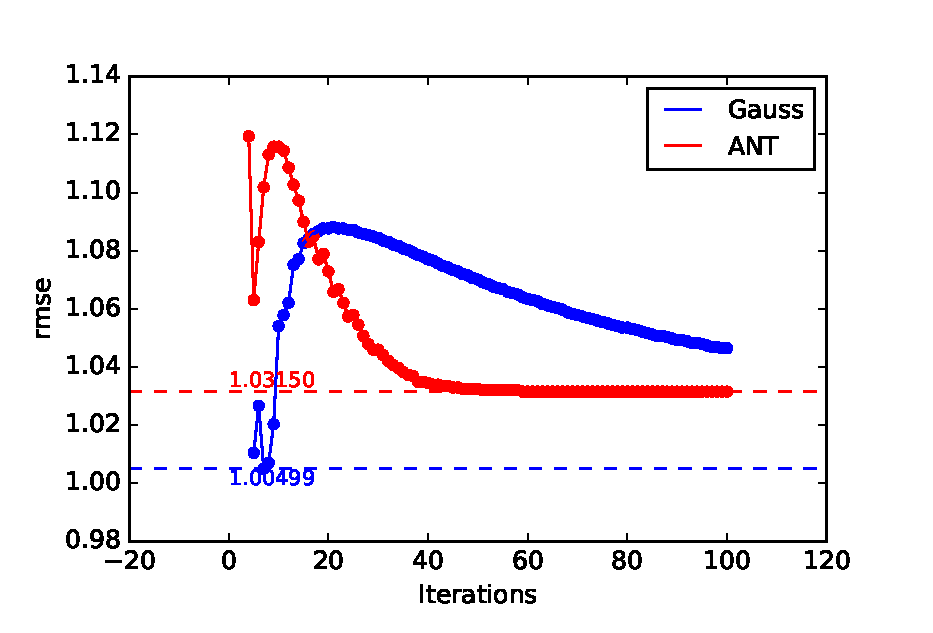
\includegraphics[width=\textwidth]{{figures/ml.0.005.rmse.iter.eps}}
                \caption{ml-10m.5e-3}
        \end{subfigure}
        \begin{subfigure}[b]{0.32\textwidth}
                \centering
                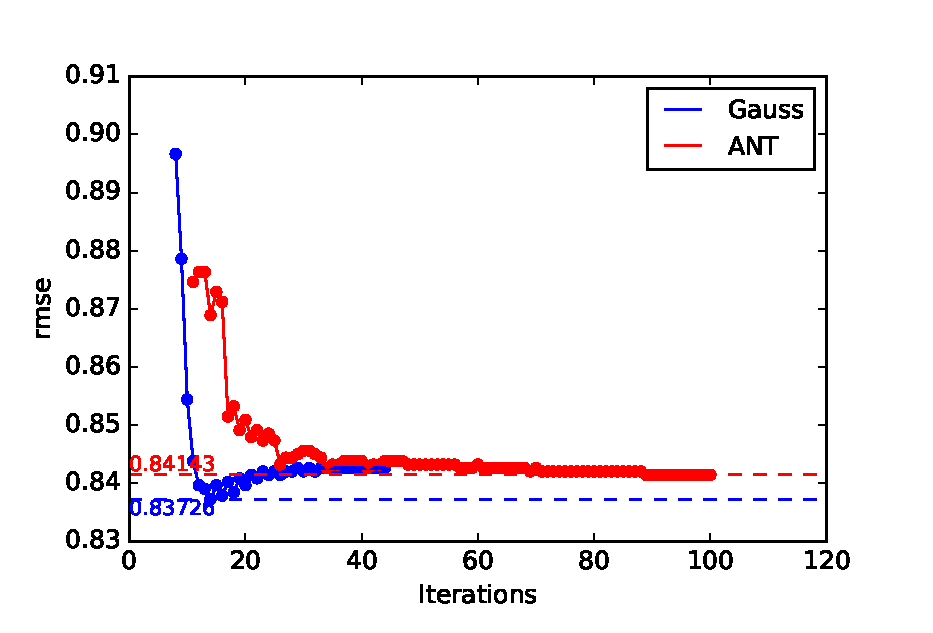
\includegraphics[width=\textwidth]{{figures/ml.0.05.rmse.iter.eps}}
                \caption{ml-10m.5e-2}
        \end{subfigure}
        \begin{subfigure}[b]{0.32\textwidth}
                \centering
                \includegraphics[width=\textwidth]{{figures/ml.0.5.rmse.iter.eps}}
                \caption{ml-10m.5e-1}
        \end{subfigure}
        \begin{subfigure}[b]{0.32\textwidth}
                \centering
                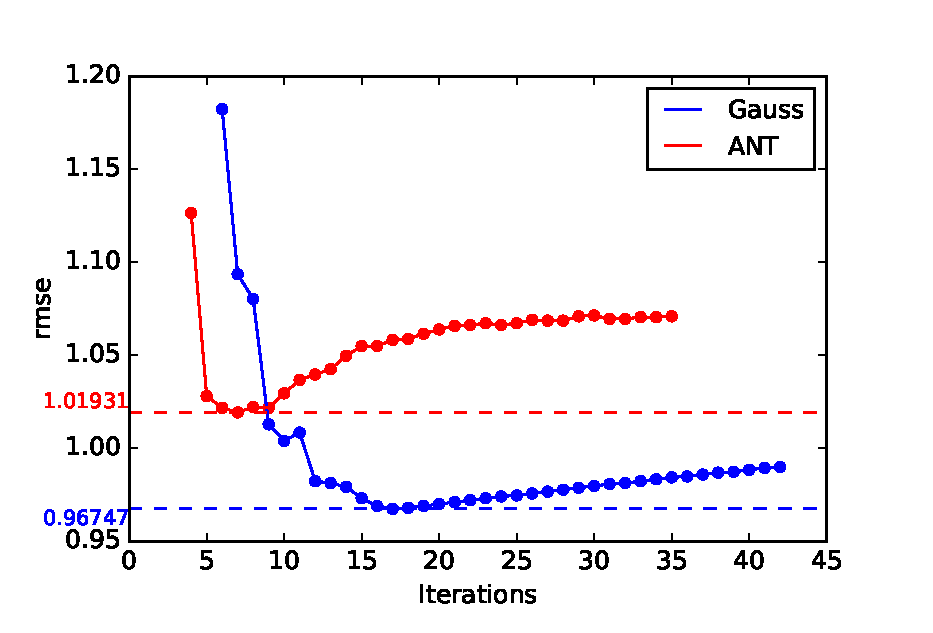
\includegraphics[width=\textwidth]{{figures/nf.0.005.rmse.iter.eps}}
                \caption{nf.5e-3}
        \end{subfigure}
        \begin{subfigure}[b]{0.32\textwidth}
                \centering
                \includegraphics[width=\textwidth]{{figures/nf.0.05.rmse.iter.eps}}
                \caption{nf.5e-2}
        \end{subfigure}
        \begin{subfigure}[b]{0.32\textwidth}
                \centering
                \includegraphics[width=\textwidth]{{figures/nf.0.5.rmse.iter.eps}}
                \caption{nf.5e-1}
        \end{subfigure}
        \caption{A comparison on the va-loss of different methods.
        The $x$-axis is the iteration,
        while the $y$-axis is the va-loss.}\label{fig:ant_gauss_valoss_iter}
\end{figure*}

\begin{figure*}[tb]
        \centering
        \begin{subfigure}[b]{0.9\textwidth}
                \centering
                \includegraphics[width=\textwidth]{{figures/ml1m_ant_valoss_iter_lambda.png}}
                \caption{Ant}
        \end{subfigure}
        \begin{subfigure}[b]{0.9\textwidth}
                \centering
                \includegraphics[width=\textwidth]{{figures/ml1m_gauss_valoss_iter_lambda.png}}
                \caption{Gauss}
        \end{subfigure}
        \caption{ml-1m. A comparison on the va-loss of different $\lambda$. 
        The $x$-axis is the iteration,
        while the $y$-axis is the va-loss.}\label{fig:ml1m_ant_gauss_valoss_iter_lambda}
\end{figure*}

\begin{figure*}[tb]
        \centering
        \begin{subfigure}[b]{0.9\textwidth}
                \centering
                \includegraphics[width=\textwidth]{{figures/ml1m_valoss_lambda.png}}
%                \caption{Ant}
        \end{subfigure}        
        \caption{ml-1m. A comparison on the best va-loss of different methods.
        The $x$-axis is $\lambda$,
        while the $y$-axis is the va-loss.}\label{fig:ml1m_ant_gauss_valoss_lambda}
\end{figure*}

%% REFERENCES

\printbibliography%

\clearpage\newpage
%\begin{algorithm}[t]
    \caption{Solving problem \eqref{eq:reMF} via alternating minimization.}
    \label{alg:AntFramework}
    \begin{algorithmic}[1]
        \State Given an initial solution $(U, V)$
        \While {stopping condition is not satisfied}
            \State $U   \gets \argmin_{U} f(U,V)$ \label{alg:AntFramework:sub_U}
            \State $V   \gets \argmin_{V} f(U,V)$
        \EndWhile
    \end{algorithmic}
\end{algorithm}

\begin{algorithm}
    \caption{Newton method for solving a sub-problem in step \ref{alg:AntFramework:sub_U} of Algorithm \ref{alg:AntFramework}.}
    \label{alg:LrFrameworkU}
    \begin{algorithmic}[1]
        \State Given $0< \epsilon < 1$, $0<\eta<1$, $\by$, $W$, $H$, and the current $U$, $V$, $f$.
        \State $Q \gets VH^T$ %, $P \gets UW^T$
        \State Compute and cache $\tilde{\by}= (Q \odot UW^T)^T\bsym{1}_{d\times 1}$.
        \State $\bb \gets \tilde{\by} - \by$
        %\State $f \gets \frac{\lambda}{2}(\|U\|_F^2 + \|V\|_F^2) + \frac{1}{2}\sum_{i=1}^l {y_i - \tilde{y}_i}$.
        %\State $f \gets \frac{\lambda}{2}(\|U\|_F^2 + \|V\|_F^2) + \frac{1}{2}\bsym{b}^T \bsym{b}$.
        \For {$k \gets \{0,1,\dots\}$}
            %\State Calculate and store $\tilde{y}_i$ and then obtain $b_i$ by \eqref{eq:LossD}, $\forall i$.
            \State Compute $G \gets \lambda U + Q \bigl(\diag(\bsym{b}) W \bigr)$
            \If {$k=0$}
                \State $\|G^0\|_F \gets \|G\|_F$
            \EndIf
            \If {$\|G\|_F \le \epsilon\|G^0\|_F$}
                \State Output $U$ as the solution of step \ref{alg:AntFramework:sub_U} in Algorithm \ref{alg:AntFramework}.
                \State {\bf break}
            \EndIf
            %\State Compute $D_{ii}$ via \eqref{eq:LossDD}, $\forall i$.
%            \State Run CG in Algorithm \ref{alg:Pcg} to get an update direction $S_u$. \label{alg:LrFrameworkU:CG}
            \State Let $S_u=\bsym{0}_{d\times M}$.
            \State Calculate $R = -G$, $D=R$, and $\gamma^0=\gamma=\|R\|_F^2$.
        \While {$\sqrt{\gamma} > \eta \sqrt{\gamma^0}$}
            %\State $\hat{D}_h \gets \hat{D} \prescript{}{\cdot}{/} \tilde{M}$
            \State $\bz \gets \left( {Q^T}\odot{(WD^T)} \right) \bsym{1}_{d\times 1}$
            \label{alg:Pcg:compz}
            \State $D_h \gets \left(\lambda D + Q \bigl(\diag(\bz) W \bigr)\right)$
            \State $\alpha \gets \gamma / \langle D,D_h \rangle$
            \State $S_u \gets S_u+\alpha D$
            \State $R \gets R-\alpha D_h$
            \State $\gamma^{\text{new}} \gets \|R\|_F^2$
            \State $\beta \gets \gamma^{\text{new}}/\gamma$
            \State $D \gets R+\beta D$
            \State $\gamma \gets \gamma^{\text{new}}$
        \EndWhile
            \State Calculate $\bsym{\Delta} = \left( Q^T \odot (WS_u^T) \right)\bsym{1}_{d\times 1}$ %, \bsym{\tilde{\Delta}}^\prime = \left( (WS_u^T) \odot (HS_v^T) \right)\bsym{1}_{d\times 1}$
%            \State Parpare the following values $\langle{U}{,}{S_u}\rangle,\|S_u\|_F^2,\text{ and } \langle{\tilde{G}}{,}{S_u}\rangle$.
            \State $\delta \gets \frac{\lambda}{2} \left( 2 \langle U, S_u \rangle + \|S_u\|_F^2 \right) + \frac{1}{2} \|\bsym{b}-\theta \Delta \|^2
                - \frac{1}{2}\bsym{b}^T \bsym{b}$
            \State $U \gets U + S_u$
            \State $f \gets f + \delta$
            \State $\tilde{\by} \gets \tilde{\by} + \theta \bsym{\Delta}$
            \State $\bb \gets \tilde{\by} - \by$

            %\State Parpare variables listed in \eqref{eq:LsRequireU} and $\bsym{\tilde{\Delta}} = \left( \pointprod{Q^T}{(WS_u^T)}+\pointprod{P^T}{(HS_v^T)} \right)\bsym{1}_{d\times 1}$
            %\For { $\theta\gets\{1,\beta,\beta^2,\dots\}$ }
            %    %\State $\delta \gets \frac{\lambda'}{2}\left( 2\theta \dotprod{U}{S} + \theta^2\|S\|_F^2 \right) +\sum_{i=1}^l \log\left(1+e^{-y_i(\tilde{y}_i+\theta\tilde{\Delta}_i)}\right)$
            %    %\vspace{-.1cm}
            %    %\Statex \hspace{1.125cm}\phantom{ $\delta \gets$}$- \sum_{i=1}^l \sum_{i=1}^l \log\left(1+e^{-y_i\tilde{y}_i}\right)$.
            %    \State $\delta \gets \frac{\lambda}{2}\left( 2\theta \langle U, S_u \rangle + 2\theta \langle V, S_v \rangle + \theta^2\|S\|_F^2 \right) + \frac{1}{2} \sum_{i=1}^l \xi(\tilde{y}_i+\theta\tilde{\Delta}_i+{\theta}^2\tilde{\Delta}_i^\prime;y_i) - \frac{1}{2}\sum_{i=1}^l \xi(\tilde{y}_i;y_i)$
            %    \If { $ \delta \le \theta \nu \langle G,S \rangle $}
            %        \State $U \gets U +\theta S_u$, $V \gets V +\theta S_v$
            %        \State $f \gets f+ \delta$
            %        \State $\bsym{\tilde{y}} \gets \bsym{\tilde{y}}+\theta\bsym{{\Delta}} +{\theta}^2 \bsym{{\Delta}}^\prime$
            %        \State {\bf break}
            %    \EndIf
            %\EndFor
        \EndFor
    \end{algorithmic}
\end{algorithm}
We consider a preconditioner $\tilde{M}$ to approximately factorize $H$ such that $H \approx \tilde{M}\tilde{M}^T$, and then use CG to solve
\begin{equation}
    \hat{H} \hat{\bs}  = \hat{\bg},
    \label{eq:PcondSys}
\end{equation}
where $\hat{H}=\tilde{M}^{-1}{H}\tilde{M}^{-T}$ and $\hat{\bg}=\tilde{M}^{-1}{\bg}$.
Once $\hat{\bs}$ is found, the solution of (\ref{eq:HLE}) can be recovered by ${\bs}=\tilde{M}^{-T}\hat{\bs}$. 
Then, we consider the following diagonal preconditioner for solving \eqref{eq:HLE} as an example.
\begin{equation}
    \tilde{M}=\tilde{M}^T=\diag({\bsym{h}}),
    \label{eq:Conder}
\end{equation}
where
\begin{equation*}
    {\bsym{h}} = \sqrt{ {\lambda} \bsym{1}_{d(M+N) \times 1} + \sum_{i=1}^l {\bj_i} \odot {\bj_i} }.
\end{equation*}
Note that ``$\sqrt{\cdot}$'' element-wisely performs the square-root operation if the input argument is a vector or a matrix. From 
\begin {align}
\bj_i &= \begin{bmatrix} \bw_i\otimes \bq_i \\ \bh_i\otimes \bp_i \end{bmatrix} = \begin{bmatrix} \vectorize(\bq_i \bw_i^T) \\ \vectorize(\bp_i \bh_i^T) \end{bmatrix}
\label{eq:Jacob_},
\end{align}
we have
\begin{align}
\sum_{i=1}^l {\bj_i} \odot {\bj_i}
&= \sum_{i=1}^l \begin{bmatrix} \vectorize \bigl((\bq_i \odot \bq_i) (\bw_i \odot \bw_i)^T \bigr) \\ \vectorize \bigl((\bp_i \odot \bp_i) (\bh_i \odot \bh_i)^T \bigr) \end{bmatrix} \nonumber  \\
&= \begin{bmatrix} \vectorize \bigl((Q \odot Q) (W \odot W) \bigr) \\ \vectorize \bigl((P \odot P) (H \odot H) \bigr) \end{bmatrix}
\label{eq:jj}.
\end{align}
Thus, the preconditioner can be obtained via
\begin{equation}
    \tilde{M}=\tilde{M}^T=\diag \Bigl( \sqrt{ {\lambda} \bsym{1}_{d(M+N) \times 1} + \begin{bmatrix} \vectorize \bigl((Q \odot Q) (W \odot W) \bigr) \\ \vectorize \bigl((P \odot P) (H \odot H) \bigr) \end{bmatrix} } \Bigr).
    \label{eq:Conder}
\end{equation}
\begin{algorithm}[t]
    \caption{A preconditioned conjugate gradient method for solving \eqref{eq:HLE} by operations on matrix variables.}
    \label{alg:PCG}
    \begin{algorithmic}[1]
        \State Given $0<\eta<1$ and $G$, the gradient matrix form of \eqref{eq:reMF}. Let $\hat{S}=\bsym{0}_{d\times (M+N)}$.
        \State Compute $M$ via \eqref{eq:Conder}.
        %\State Calculate $\hat{G} = G \prescript{}{\cdot}{/} M$, $R=-\hat{G}$, $\gamma=\no{R}_F^2$, and $\hat{D}=R$.
        \State Calculate $R = -G\prescript{}{\cdot}{/} M$, $\hat{D}=R$, and $\gamma^0=\gamma=\|R\|_F^2$.
        \While {$\sqrt{\gamma} > \eta \sqrt{\gamma^0}$}
            \State $\hat{D}_h \gets \hat{D}\prescript{}{\cdot}{/} M $
            \State $\hat{\bz}\gets \left( {Q^T}\odot{(W\hat{D}_{hu}^T)}+{P^T}\odot{(H\hat{D}_{hv}^T)} \right) \bsym{1}_{d\times 1}$
            \State $\hat{D}_h \gets \left(\lambda \hat{D}_h + \begin{bmatrix} Q \bigl(\diag(\hat{\bz}) W \bigr) \, P \bigl ( \diag(\hat{\bz}) H \bigr) \end{bmatrix}\right)\prescript{}{\cdot}{/} M $
            \State $\alpha \gets \gamma / \langle \hat{D},\hat{D}_h \rangle$
            \State $\hat{S} \gets\hat{S}+\alpha \hat{D}$
            \State $R \gets R-\alpha \hat{D}_h$
            \State $\gamma^{\text{new}} \gets \|R\|_F^2$
            \State $\beta \gets \gamma^{\text{new}}/\gamma$
            \State $\hat{D} \gets R+\beta \hat{D}$
            \State $\gamma \gets \gamma^{\text{new}}$
        \EndWhile
        \State Output $S=\hat{S}\prescript{}{\cdot}{/} M$ as the solution.
    \end{algorithmic}
\end{algorithm}

\end{document}

%%% Local Variables: ***
%%% mode:latex ***
%%% End: ***
